\documentclass[9pt,a4paper]{report}
\usepackage{amsfonts,amsmath,amsthm,amssymb,graphicx,graphics,tikz,xcolor}
\usepackage{indentfirst,enumerate,wrapfig,caption,multirow,cite,tabularx}
\usepackage{algorithm,algorithmicx,algpseudocode}
\usepackage[colorlinks=true,citecolor=blue,linkcolor=black,urlcolor=black,bookmarks=true]{hyperref}
\usepackage[utf8x]{inputenc}
\renewcommand{\figurename}{Figura}
\renewcommand{\chaptername}{Capitolul}
\renewcommand{\bibname}{Bibliografie}
\renewcommand{\contentsname}{Cuprins}
\renewcommand{\citeleft}{\textcolor{blue}{[}}
\renewcommand{\citeright}{\textcolor{blue}{]}}
\newcommand*\nod[1]{\tikz[baseline=(char.base)]{\node[shape=circle,draw,inner sep=1pt] (char) {#1};}}
\newcommand\grafsus[1]{\raisebox{-0.9\totalheight}{#1}}
\newtheorem{definitie}{Definiția}
\newtheorem{teorema}{Teorema}
\usetikzlibrary{matrix}

\begin{document}

\thispagestyle{empty}

\begin{center}
    \bfseries

    \Huge
    INTRODUCERE ÎN \\
    TEORIA GRAFURILOR
    \vspace{25pt}

    \normalsize
    CÂTEVA CONSIDERAȚII ASUPRA CONCEPTELOR \\
    ESENȚIALE CARE STAU LA BAZA TEORIEI GRAFURILOR \\
    ȘI ALGORITMILOR FUNDAMENTALI UTILIZAȚI ÎN \\
    REZOLVAREA PROBLEMELOR COMPUTAȚIONALE \\
    \vspace{25pt}

    \includegraphics[width=0.9\textwidth]{img/cayley_graph} \\
    \textnormal{\textit{Un graf Cayley pentru $C_3 * C_5$.}}
    \vspace{25pt}

    \small
    DE\\

    \Large
    SÎRBU MATEI-DAN \\
    \href{mailto:hello@msirbu.eu}{hello@msirbu.eu} \\
    \vspace{25pt}

    BRAȘOV, DECEMBRIE 2020
\end{center}

\newpage

\tableofcontents
\thispagestyle{empty}

\newpage
\setcounter{page}{1}

\chapter{Despre conceptul de \textit{graf}}
\section{Terminologie}

Definim în mod informal un graf ca fiind o colecție de ,,noduri'' unite prin ,,muchii'', ca în exemplul\textsuperscript{\cite{gabow}} următor:

\begin{figure}[htbp]
    \centering
    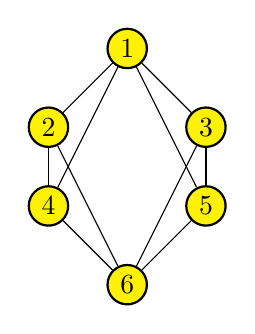
\begin{tikzpicture}[every node/.style={draw=black,thick,circle,inner sep=0pt,fill=yellow,minimum size=0.5cm}]
        \node (1) at (0,0) {1};
        \node (2) at (-1,-1) {2};
        \node (3) at (1,-1) {3};
        \node (4) at (-1,-2) {4};
        \node (5) at (1,-2) {5};
        \node (6) at (0,-3) {6};

        \path [-] (1) edge (3);
        \path [-] (1) edge (4);
        \path [-] (1) edge (5);
        \path [-] (2) edge (4);
        \path [-] (1) edge (2);
        \path [-] (2) edge (6);
        \path [-] (3) edge (5);
        \path [-] (3) edge (6);
        \path [-] (4) edge (6);
        \path [-] (5) edge (6);
    \end{tikzpicture}
    \caption{Un graf neorientat oarecare.}
    \label{fig:graf1}
\end{figure}

\begin{definitie}
    Un \textbf{graf} este o pereche $(V,E)$, unde $V$ este o mulțime finită de elemente, numite \textit{noduri (\textbf{V}ertices)}, iar $E$ este o mulțime finită de perechi de noduri, numite \textit{muchii (\textbf{E}dges)}.
\end{definitie}

Dacă perechile din mulțimea $E$ sunt ordonate, atunci spunem că graful este \textbf{\textit{orientat}}, sau \textbf{\textit{digraf}}; în caz contrar, graful este \textbf{\textit{neorientat}}. De asemenea, două noduri unite de o muchie se numesc \textit{\textbf{adiacente}}. Conceptul analog muchiilor aplicabil grafurilor orientate este \textbf{\textit{arcul}}.

\section{Dimensiunile unui graf}

De obicei, notăm cu $n$ numărul de noduri ale unui graf; mai precis, $n = |V|$. Cu $m$ vom nota numărul de muchii, adică $m = |E|$. În graful din figura \ref{fig:graf1}, $n$ este 6, iar $m$ este 10.

\begin{teorema}
    Dacă un graf neorientat are $n$ noduri, atunci \textbf{\textit{numărul total de grafuri neorientate}}\textsuperscript{\cite{milosescu}} care se pot forma cu aceste noduri este $g = 2^{C_n^2}$.
\end{teorema}

\begin{teorema}
    Graful \textbf{\textit{complet}}, graful care are toate muchiile posibile, conține $m = \frac{n(n-1)}{2}$ muchii\textsuperscript{\cite{milosescu}}, dacă este neorientat.
\end{teorema}

Spunem despre un nod că este \textbf{\textit{izolat}} dacă nu aparține niciunei muchii. Întrucât nodurile izolate sunt inutile în majoritatea aplicațiilor, presupunem că nu există astfel de noduri; în acest caz, știm despre numărul de muchii că este $m \geq \frac{n}{2}$.

Astfel, deducem, utilizând simbolul O al lui Landau (notația \textit{big-O}), că în general, $m = O(n^2)$, iar în majoritatea aplicațiilor, $m = \Omega(n)$, limite care sunt aplicabile și digrafurilor. Din punct de vedere terminologic, grafurile cu $m = \Theta(n)$ se numesc \textbf{\textit{rare}}, iar cele cu $m = \Theta(n^2)$ sunt \textbf{\textit{dense}}\textsuperscript{\cite{gabow}}.

\section{Conexitate}

\begin{definitie}
    Un \textbf{subgraf} $G' = (V', E')$ este un subgraf al lui $G = (V, E)$ dacă $V' \subseteq V$ și $E' \subseteq E$.
\end{definitie}
\begin{definitie}
    Un \textbf{lanț} este o succesiune de noduri $v_0, v_1, \dots, v_l$, $l \geq 0$, cu $(v_i, v_{i+1}) \in E$ pentru $i = \overline{0, \ l - 1}$. Analog, în cazul grafurilor orientate, această succesiune de noduri se numește \textbf{drum}.
\end{definitie}

Un lanț este \textbf{\textit{simplu}} dacă nu trece de două ori prin aceeași muchie. În caz contrar, se numește lanț \textbf{\textit{compus}}. Este de remarcat faptul că un lanț poate avea lungime nulă.

\begin{definitie}
    Un \textbf{ciclu} este un drum cu $l \geq 3$, $v_0 = v_l$ cu toate nodurile și muchiile distincte.
\end{definitie}

\begin{definitie}
    \textbf{Gradul} unui nod $v_k$ al grafului $G$ este egal cu numărul muchiilor incidente cu nodul și se notează cu $d(v_k)$.
\end{definitie}

\begin{teorema}
    Dacă graful $G$ are $m$ muchii și $n$ noduri, atunci între \textbf{gradul nodurilor} și \textbf{numărul de muchii} există relația\textsuperscript{\cite{milosescu}} $\sum_{i=1}^n d(v_i) = 2m$.
\end{teorema}

În funcție de gradul nodurilor putem distinge câteva cazuri particulare\textsuperscript{\cite{milosescu}}. Un \textbf{\textit{nod terminal}} este incident cu o singură muchie, adică $d(v_k) = 1$. Un \textbf{\textit{nod izolat}} nu este adiacent cu nici un alt nod al grafului, adică nu se găsește în extremitatea niciunei muchii; altfel spus, $d(v_k) = 0$. Un exemplu\textsuperscript{\cite{milosescu}}:

\begin{center}
    \begin{minipage}[t]{0.5\textwidth}
        \vspace{0pt} % force top alignment when using text and figure
        Graful $G = (V, E)$ din figură este definit astfel:
        \begin{itemize}
            \item $V = \{1, 2, 3, \dots, 11\}$
            \item $E = \{(1,2), (1,4), (2,3), (2,5), \\ (3,4), (3,5), (5,6), (5,7), (5,8), (7,9)\}$
        \end{itemize}
        Despre graful $G$ putem spune că:
    \end{minipage}
    \begin{minipage}[t]{0.49\textwidth}
        \vspace{0pt}
        \begin{flushright}
            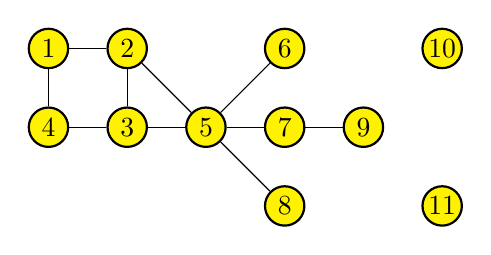
\begin{tikzpicture}[every node/.style={draw=black,thick,circle,inner sep=0pt,fill=yellow,minimum size=0.5cm}]
                \node (1) at (0,0) {1};
                \node (2) at (1,0) {2};
                \node (3) at (1,-1) {3};
                \node (4) at (0,-1) {4};
                \node (5) at (2,-1) {5};
                \node (6) at (3,0) {6};
                \node (7) at (3,-1) {7};
                \node (8) at (3,-2) {8};
                \node (9) at (4,-1) {9};
                \node (10) at (5,0) {10};
                \node (11) at (5,-2) {11};

                \path [-] (1) edge (2);
                \path [-] (1) edge (4);
                \path [-] (2) edge (3);
                \path [-] (2) edge (5);
                \path [-] (3) edge (4);
                \path [-] (3) edge (5);
                \path [-] (5) edge (6);
                \path [-] (5) edge (7);
                \path [-] (5) edge (8);
                \path [-] (7) edge (9);
            \end{tikzpicture}
        \end{flushright}
    \end{minipage}
\end{center}

\begin{itemize}
    \item $d(v_5) = 5$, deoarece \nod{5} are 5 muchii incidente: $(2,5), (3,5), (5,6), (5,7)$ și $(5,8)$.
    \item $d(v_9) = 1$, adică \nod{9} este \textit{nod terminal}, deoarece are o singură muchie incidentă: $(7,9)$.
    \item $d(v_{10}) = 0$, adică \nod{10} este \textit{nod izolat}, deoarece nu are muchii incidente.
\end{itemize}

\begin{definitie}
    Un graf neorientat este \textbf{conex} dacă are un lanț care unește oricare două noduri.
\end{definitie}
\begin{definitie}
    Un \textbf{arbore} este un graf neorientat conex fără cicluri.
\end{definitie}
\begin{definitie}
    Un \textbf{arbore de acoperire}\textsuperscript{\cite{gabow}} este un subgraf al unui graf neorientat conex care conține toate nodurile din graf.
\end{definitie}

\begin{figure}[htbp]
    \begin{minipage}{0.5\textwidth}
        \centering \vspace{0pt}
        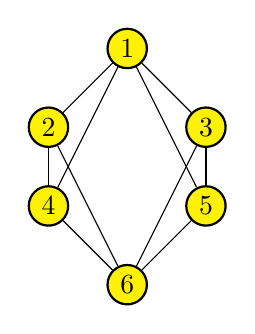
\begin{tikzpicture}[every node/.style={draw=black,thick,circle,inner sep=0pt,fill=yellow,minimum size=0.5cm}]
            \node (1) at (0,0) {1};
            \node (2) at (-1,-1) {2};
            \node (3) at (1,-1) {3};
            \node (4) at (-1,-2) {4};
            \node (5) at (1,-2) {5};
            \node (6) at (0,-3) {6};

            \path [-] (1) edge (3);
            \path [-] (1) edge (4);
            \path [-] (1) edge (5);
            \path [-] (2) edge (4);
            \path [-] (1) edge (2);
            \path [-] (2) edge (6);
            \path [-] (3) edge (5);
            \path [-] (3) edge (6);
            \path [-] (4) edge (6);
            \path [-] (5) edge (6);
        \end{tikzpicture}
    \end{minipage}
    \begin{minipage}{0.49\textwidth}
        \centering \vspace{0pt}
        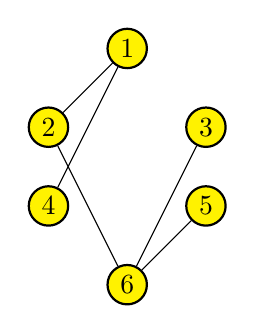
\begin{tikzpicture}[every node/.style={draw=black,thick,circle,inner sep=0pt,fill=yellow,minimum size=0.5cm}]
            \node (1) at (0,0) {1};
            \node (2) at (-1,-1) {2};
            \node (3) at (1,-1) {3};
            \node (4) at (-1,-2) {4};
            \node (5) at (1,-2) {5};
            \node (6) at (0,-3) {6};

            \path [-] (1) edge (4);
            \path [-] (1) edge (2);
            \path [-] (2) edge (6);
            \path [-] (3) edge (6);
            \path [-] (5) edge (6);
        \end{tikzpicture}
    \end{minipage}
    \caption{Arborele din fig. \ref{fig:graf1}, respectiv arborele de acoperire al acestuia.}
    \label{fig:graf2}
\end{figure}

Într-un graf orientat, un arc $(u,v)$ pornește din \nod{$u$} și ajunge în \nod{$v$}; \nod{$v$} se numește \textit{\textbf{capul}} arcului, iar \nod{$u$} este \textit{\textbf{coada}}. \nod{$v$} este accesibil din \nod{$u$} dacă și numai dacă există un drum de la \nod{$u$} la \nod{$v$}. O remarcă importantă este aceea că \textit{\textbf{buclele}}, $(u, u)$, sunt permise în grafurile orientate, dar nu și în cele neorientate.

\section{Operații pe grafuri}
În tabelul următor\textsuperscript{\cite{gabow}} vor fi enumerate operațiile de bază care pot fi executate pe grafuri, și rezultatul aplicării acestora pe graful din figura \ref{fig:graf1}, notat aici cu $G$. \\

\noindent
\begin{tabularx}{\linewidth}{Xr}
    \textbf{Operația pe graf}                                                            & \textbf{Graful rezultat} \\ \hline
    Ștergerea unei muchii din $G$ înseamnă formarea grafului $G - e$.
    \newline\newline \textbf{Exemplu:} $e = \{(2,4),(3,5)\}$                             & \grafsus{
        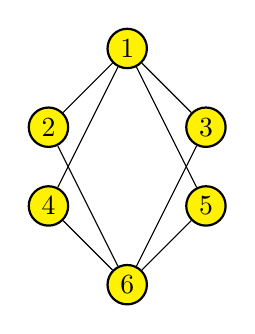
\begin{tikzpicture}[every node/.style={draw=black,thick,circle,inner sep=0pt,fill=yellow,minimum size=0.5cm}]
            \node (1) at (0,0) {1};
            \node (2) at (-1,-1) {2};
            \node (3) at (1,-1) {3};
            \node (4) at (-1,-2) {4};
            \node (5) at (1,-2) {5};
            \node (6) at (0,-3) {6};

            \path [-] (1) edge (2);
            \path [-] (1) edge (3);
            \path [-] (1) edge (4);
            \path [-] (1) edge (5);
            \path [-] (2) edge (6);
            \path [-] (3) edge (6);
            \path [-] (4) edge (6);
            \path [-] (5) edge (6);
        \end{tikzpicture}}
    \\ \hline
    Ștergerea unei nod din $G$ determină formarea grafului $G - v$; presupune păstrarea tuturor nodurilor și muchiilor din $G$
    cu excepția nodurilor din $v$ și a muchiilor incidente acestora
    \newline\newline \textbf{Exemplu:} $v = \{6\}$; formează un ,,\textit{graf papion}'' & \grafsus{
        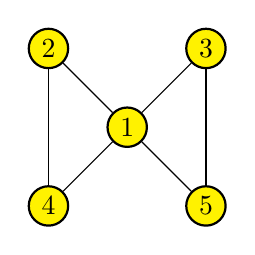
\begin{tikzpicture}[every node/.style={draw=black,thick,circle,inner sep=0pt,fill=yellow,minimum size=0.5cm}]
            \node (1) at (0,0) {1};
            \node (2) at (-1,1) {2};
            \node (3) at (1,1) {3};
            \node (4) at (-1,-1) {4};
            \node (5) at (1,-1) {5};

            \path [-] (1) edge (3);
            \path [-] (1) edge (4);
            \path [-] (1) edge (5);
            \path [-] (2) edge (4);
            \path [-] (1) edge (2);
            \path [-] (3) edge (5);
        \end{tikzpicture}}
    \\ \hline
\end{tabularx}

\noindent
\begin{tabularx}{\linewidth}{Xr}
    \textbf{Operația pe graf}                               & \textbf{Graful rezultat} \\ \hline
    Contractarea unei mulțimi de noduri $S$ determină formarea grafului $G - S$, unde mulțimea $S$ este
    înlocuită de un nou nod \nod{$\Sigma$}, adiacent tuturor vecinilor nodurilor din $S$
    \newline\newline \textbf{Exemplu:} $\Sigma = \{4,5,6\}$ & \grafsus{
        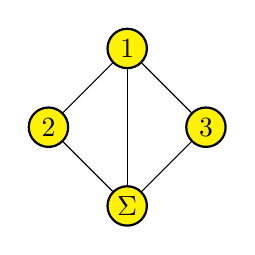
\begin{tikzpicture}[every node/.style={draw=black,thick,circle,inner sep=0pt,fill=yellow,minimum size=0.5cm}]
            \node (1) at (0,1) {1};
            \node (2) at (-1,0) {2};
            \node (3) at (1,0) {3};
            \node (S) at (0,-1) {$\Sigma$};

            \path [-] (1) edge (2);
            \path [-] (1) edge (3);
            \path [-] (1) edge (S);
            \path [-] (2) edge (S);
            \path [-] (3) edge (S);
        \end{tikzpicture}}
    \\ \hline
\end{tabularx}

\section{Reprezentarea grafurilor}
Există mai multe moduri de reprezentare la nivel logic a unui graf\textsuperscript{\cite{milosescu}}, care pot fi implementate în memoria unui calculator, folosind diverse tipuri de structuri de date. Aceste reprezentări pot fi folosite în algoritmii care prelucrează grafuri și, implicit, în programele prin care vor fi implementați în calculator acești algoritmi. Printre modurile de reprezentare a unui graf se numără:
\begin{itemize}
    \item reprezentarea prin \textbf{\textit{matricea de adiacență}};
    \item reprezentarea prin \textbf{\textit{lista muchiilor (arcelor)}};
    \item reprezentarea prin \textbf{\textit{lista de adiacență (listele vecinilor)}};
    \item reprezentarea prin \textbf{\textit{matricea costurilor}}.
\end{itemize}

Fiecare reprezentare prezintă avantaje în ceea ce privește utilizarea eficientă a memoriei interne, în funcție de tipul grafului (cu noduri puține, dar cu muchii multe - sau cu noduri multe, dar cu muchii puține) și din punct de vedere al eficienței algoritmilor de prelucrare (în funcție de aplicație). În următoarele reprezentări se consideră că graful $G = (V, E)$ are $n$ noduri și $m$ muchii.

\subsection{Matricea de adiacență}

\begin{definitie}
    \textbf{Matricea de adiacență}\textsuperscript{\cite{milosescu}} a unui graf este o matrice pătratică binară de ordinul $n$ ($A_{n,n}$), ale cărei elemente $a_{i,j}$ sunt definite astfel:
    $$
        a_{i,j} =
        \begin{cases}
            1, & \text{\normalfont{dacă }} [i, j] \in E    \\
            0, & \text{\normalfont{dacă }} [i, j] \notin E \\
        \end{cases}.
    $$
\end{definitie}

\begin{figure}[htbp]
    \centering
    \includegraphics[width=0.3\textwidth]{img/adjacency_matrix.png}
    \label{fig:graf3}
    \caption{Matricea de adiacență a grafului din fig. \ref{fig:graf1}}
\end{figure}

În cazul grafurilor orientate putem diferenția gradul unui nod:
\begin{definitie}
    \textbf{Gradul intern} al unui nod $v_i$ al grafului $G$ este egal cu numărul arcelor care intră în nodul $v_i$ și se notează cu $d^-(v)$.
\end{definitie}
\begin{definitie}
    \textbf{Gradul extern} al unui nod $v_i$ al grafului $G$ este egal cu numărul arcelor care ies din nodul $v_i$ și se notează cu $d^+(v)$.
\end{definitie}

Pentru a calcula gradul extern al unui digraf reprezentat ca o matrice de adiacență vom utiliza următorul algoritm\textsuperscript{\cite{gabow}}, care are complexitatea de timp $\Theta(n^2)$:

\begin{algorithm}
    \begin{algorithmic}
        \Procedure{grad-extern}{$A, v$}
        \For{$v \gets 1$ \textbf{to} {$n$}}
        \State {$d[v] \gets 0$}
        \For{$w \gets 1$ \textbf{to} {$n$}}
        \State {$d[v] \gets d[v] + A[v,w]$}
        \EndFor
        \EndFor
        \EndProcedure
    \end{algorithmic}
\end{algorithm}

\subsubsection*{Proprietăți}

\begin{itemize}
    \item Elementele de pe diagonala principală au valoarea 0. Din definiția grafului rezultă că orice muchie/arc $(i,j)$ trebuie să respecte condiția $i \neq j$.
\end{itemize}

Pentru grafurile neorientate:

\begin{itemize}
    \item Matricea de adiacență este o matrice simetrică față de diagonala principală, deoarece, dacă există muchia $(i, j)$, atunci există și muchia $(j, i)$.
    \item Suma elementelor matricei de adiacență este egală cu $2m$.
    \item Gradul unui nod $i$ este egal cu suma elementelor de pe linia $i$.
    \item Nodurile adiacente nodului $i$ sunt nodurile $j$ pentru care elementele din linia $i$ sunt egale cu 1. Mai pot fi definite ca nodurile $j$ pentru care elementele din coloana $i$ sunt egale cu 1.
    \item Numărul de vecini ai nodului $i$ este egal cu gradul nodului.
    \item Muchia $(i,j)$ a grafului reprezintă un element al matricei de adiacență care îndeplinește condiția $a_{i,j}=a_{j,i}=1$
\end{itemize}

Pentru grafurile orientate:

\begin{itemize}
    \item Suma elementelor matricei de adiacență ete egală cu $m$.
    \item Gradul extern al nodului $i$ este egal cu suma elementelor de pe linia $i$.
    \item Gradul intern al nodului $i$ este egal cu suma elementelor de pe coloana $i$.
    \item Succesorii nodului $i$ sunt nodurile $j$ pentru care elementele din linia $i$ sunt egale cu 1.
    \item Predecesorii nodului $i$ sunt nodurile $j$ pentru care elementele din coloana $i$ sunt egale cu 1.
    \item Nodurile adiacente nodului $i$ sunt nodurile $j$ pentru care elementele din linia $i$ sau din coloana $i$ sunt egale cu 1, sau reuniunea dintre mulțimea succesorilor și mulțimea predecesorilor nodului.
    \item Numărul de vecini ai nodului $i$ este egal cu cardinalul mulțimii de noduroi adiacente nodului $i$.
    \item Arcul $(i,j)$ al grafului reprezintă un element al matricei de adiacență care îndeplinește condiția $a_{i,j}=1$.
\end{itemize}

\subsection{Lista muchiilor (arcelor)}

\begin{definitie}
    \textbf{Lista muchiilor}\textsuperscript{\cite{milosescu}} unui graf este formată din $m$ elemente care conțin, fiecare, câte o pereche de două noduri, $v_i$ și $v_j$, care formează o muchie, adică pentru care $(v_i,v_j) \in E$.
\end{definitie}

Lista de muchii care descrie graful din figura \ref{fig:graf1} este:
$$L = \{(1,2),(1,3),(1,4),(1,5),(2,4),(2,6),(3,5),(3,6),(4,6),(5,6)\}.$$

\subsubsection*{Proprietăți}

Pentru grafurile neorientate:

\begin{itemize}
    \item Graful unui nod $i$ este egal cu numărul de apariții ale etichetei nodului în câmpurile vectorului de înregistrări.
    \item Nodurile adiacente nodului $i$ sunt etichetele $j$ din câmpul $L_{k,1}$, pentru care $L_{k,0} = i$, sau de pe al doilea câmp, pentru care $L_{k,2} = i$.
    \item Numărul de vecini ai nodului $i$ este egal cu gradul nodului.
\end{itemize}

Pentru grafurile orientate:

\begin{itemize}
    \item Gradul extern al nodului $i$ este egal cu numărul de apariții ale etichetei nodului în primul câmp în vectorul de înregistrări.
    \item Gradul intern al nodului $i$ este egal cu numărul de apariții ale etichetei nodului în al doilea câmp în vectorul de înregistrări.
    \item Succesorii nodului $i$ sunt etichetele $j$ din câmpul $L_{k,2}$ pentru care $L_{k,1} = i$.
    \item Predecesorii nodului $i$ sunt etichetele $j$ din câmpul $L_{k,1}$ pentru care $L_{k,2} = i$.
    \item Nodurile adiacente nodului $i$ sunt date de reuniunea dintre mulțimea succesorilor și mulțimea predecesorilor nodului.
\end{itemize}

\subsection{Lista de adiacență}

\begin{definitie}
    \textbf{Lista de adiacență}\textsuperscript{\cite{milosescu}} este formată din listele $L_i$ $(1 \leq i \leq n)$ care conțin toți vecinii unui nod $v_i$ la care se poate ajunge direct din nodul $v_i$, adică toate nodurile $v_j$ pentru care $(v_i, v_j) \in E$.
\end{definitie}

\begin{figure}[htbp]
    \centering
    \includegraphics[width=0.6\textwidth]{img/adjacency_lists.png}
    \label{fig:graf3}
    \caption{Listele de adiacență care definesc graful din fig. \ref{fig:graf1}}
\end{figure}

\subsubsection*{Proprietăți}

Pentru grafurile neorientate:

\begin{itemize}
    \item Numărul de elemente din toate listele simplu înlănțuite este egal cu $2m$.
    \item Lungimea listei de adiacență a nodului $i$ este egală cu numărul de noduri ale listei ce are adresa nodului prim egală cu $L_i$.
    \item Graful unui nod $i$ sunt nodurile a căror etichetă apare în lista ce are adresa nodului prim egală cu $L_i$.
    \item Numărul de vecini ai nodului $i$ este egal cu gradul nodului.
    \item Muchia $(i,j)$ a grafului reprezintă nodul $i$ și un nod $j$ din lista ce are adresa nodului prim egală cu $L_i$.
\end{itemize}

Pentru grafurile orientate:

\begin{itemize}
    \item Numărul de elemente din toate listele simplu înlănțuite este egal cu $m$.
    \item Lungimea listei de adiacență $i$ este egală cu numărul de noduri ale listei care are adresa nodului prim egală cu $L_i$.
    \item Gradul extern al nodului $i$ este egal cu lungimea listei de adiacență a nodului.
    \item Gradul intern al nodului $i$ este egal cu numărul de apariții ale etichetei nodului în toate listele simplu înlănțuite.
    \item Succesorii nodului $i$ sunt nodurile a căror etichetă apare în lista ce are adresa nodului prim egală cu $L_i$.
    \item Predecesorii nodului $i$ sunt nodurile $j$ în ale căror liste, ce au adresa nodului prim egală cu $L_j$, apare nodului $i$.
    \item Nodurile adiacente nodului $i$ sunt date de reuniunea dintre mulțimea succesorilor și mulțimea predecesorilor nodului.
    \item Numărul de vecini ai nodului $i$ este egal cu cardinalul mulțimii de noduri adiacente nodului $i$.
    \item Arcul $(i,j)$ al grafului reprezintă nodul $i$ și un nod $j$ din lista ce are adresa nodului prim egală cu $L_i$.
\end{itemize}

\subsection{Matricea costurilor}

\begin{definitie}
    \textbf{Graful ponderat}, este graful $G=(V, E)$ pentru care s-a definit o funcție $f : E \rightarrow \mathbb{R}_+$ care asociază fiecărei muchii/arc $e$ un număr real pozitiv (care poate avea semnificația de cost, distanță, timp, durată), numită în general \textbf{costul muchiei}, sau \textbf{funcția cost}.
\end{definitie}

\begin{definitie}
    \textbf{Matricea costurilor}\textsuperscript{\cite{milosescu}} unui graf este o matrice pătratică de dimensiune $n$ ($A_{n,n}$) ale cărei elemente $a_{i,j}$ sunt definite astfel încât să pună în evidență costul asociat fiecărei muchii/arc.
\end{definitie}

\begin{figure}[htbp]
    \centering
    \begin{minipage}[t]{0.49\textwidth}
        \begin{center}
            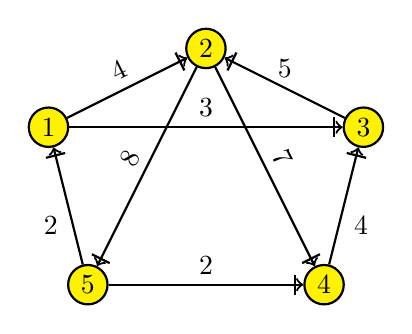
\begin{tikzpicture}[nod/.style={draw=black,thick,circle,inner sep=0pt,fill=yellow,minimum size=0.5cm}]
                \node[nod] (1) at (-2,-1) {1};
                \node[nod] (2) at (0,0) {2};
                \node[nod] (3) at (2,-1) {3};
                \node[nod] (4) at (1.5,-3) {4};
                \node[nod] (5) at (-1.5,-3) {5};

                \draw [thick, -|>] (1) -- (2) node[midway, sloped, above] {4};
                \draw [thick, -|>] (1) -- (3) node[midway, above] {3};
                \draw [thick, -|>] (2) -- (5) node[midway, sloped, above] {8};
                \draw [thick, -|>] (2) -- (4) node[midway, sloped, above] {7};
                \draw [thick, -|>] (3) -- (2) node[midway, above] {5};
                \draw [thick, -|>] (5) -- (1) node[midway, below left] {2};
                \draw [thick, -|>] (5) -- (4) node[midway, sloped, above] {2};
                \draw [thick, -|>] (4) -- (3) node[midway, below right] {4};
            \end{tikzpicture}
        \end{center}
    \end{minipage}
    \begin{minipage}[t]{0.5\textwidth}
        \begin{center}
            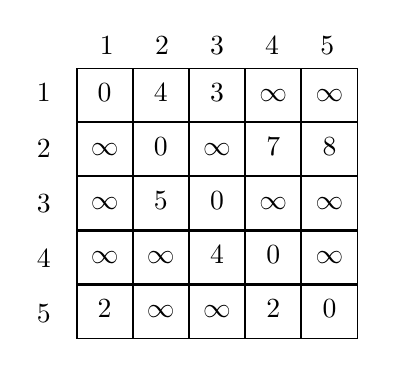
\begin{tikzpicture}
                \node at (-1.4,2) {1};
                \node at (-0.7,2) {2};
                \node at (0,2) {3};
                \node at (0.7,2) {4};
                \node at (1.4,2) {5};
                \node at (-2.2,1.4) {1};
                \node at (-2.2,0.7) {2};
                \node at (-2.2,0) {3};
                \node at (-2.2,-0.7) {4};
                \node at (-2.2,-1.4) {5};
                \matrix[matrix of nodes,nodes in empty cells,nodes={draw,text depth=.14cm, text height=.3cm, minimum width=.7cm}]
                {
                    0        & 4        & 3        & $\infty$ & $\infty$ \\
                    $\infty$ & 0        & $\infty$ & 7        & 8        \\
                    $\infty$ & 5        & 0        & $\infty$ & $\infty$ \\
                    $\infty$ & $\infty$ & 4        & 0        & $\infty$ \\
                    2        & $\infty$ & $\infty$ & 2        & 0        \\
                };
            \end{tikzpicture}
        \end{center}
    \end{minipage}
    \caption{Un graf ponderat, respectiv matricea sa de costuri.}
    \label{fig:graf4}
\end{figure}

Pentru a crea matricea costurilor trebuie să se citească pentru fiecare muchie (arc) nodurile de la extremități și costul asociat fiecărei muchii (arc). Aceste informații se pot citi de la tastatură sau dintr-un fișier. Algoritmul pentru crearea matricii costurilor este:

\begin{enumerate}
    \item Se inițializează matricea astfel: toate elementele de pe diagonala principală cu valoarea 0, iar restul elementelor cu valoarea corespunzătoare pentru $\infty$ ($-\infty$).
    \item Se actualizează matricea cu informațiile despre costurile asociate muchiilor (arcelor) astfel: pentru fiecare muchie (arc) $(i,j)$ cu costul $c$, elementului $a_{i,j}$ i se va atribui valoarea costului $c$.
\end{enumerate}

\chapter{Algoritmi esențiali}

O mare varietate de probleme se formulează în termeni de grafuri. Pentru a le rezolva, de multe ori trebuie să explorăm un graf, adică să consultăm (vizităm) vârfurile sau muchiile grafului respectiv. Uneori trebuie să consultăm toate vârfurile sau muchiile, alteori trebuie să consultăm doar o parte din ele. 

În acest capitol, introducem câteva tehnici care pot fi folosite atunci când nu este specificată o anumită ordine a consultărilor. Indiferent de obiectivul urmărit, explorarea se realizează pe baza unor algoritmi de parcurgere, care asigură consultarea sistematică a vârfurilor sau muchiilor grafului respectiv.

\section{Depth-First Search}

Fie $G = (V, E)$ un graf orientat sau neorientat, ale cărui vârfuri dorim să le consultăm. Presupunem că avem posibilitatea să marcăm vârfurile deja vizitate în tabloul global $marca$. Inițial, nici un vârf nu este marcat.
Pentru a efectua o parcurgere în adâncime, alegem un vârf oarecare, $v \in V$, ca punct de plecare și îl marcăm. Dacă există un vârf $w$ adiacent lui $v$ (adică, dacă există muchia $(v, w)$ în graful G) care nu a fost vizitat, alegem vârful $w$ ca noul punct de plecare și apelăm recursiv procedura de parcurgere în adâncime. La întoarcerea din apelul recursiv, dacă există un alt vârf adiacent lui $v$ care nu a fost vizitat, apelăm din nou procedura etc. 

Când toate vârfurile adiacente lui $v$ au fost marcate, se încheie consultarea începută în $v$. Dacă au rămas vârfuri în $V$ care nu au fost vizitate, alegem unul din aceste vârfuri și apelăm procedura de parcurgere. Continuăm astfel, până când toate vârfurile din $V$ au fost marcate. 

Algoritmul de parcurgere (DFS)\textsuperscript{\cite{andonie}} a grafurilor în adâncime este prezentat mai jos:

\pagebreak

\begin{algorithm}
    \begin{algorithmic}
        \Procedure{parcurge}{$G$}\Comment{Parcurgerea în adâncime}
            \For{fiecare $v \in V$}
                \State{$marca[v] \gets \text{nevizitat}$}
            \EndFor
            \For{fiecare $v \in V$}
                \If{$marca[v] = \text{nevizitat}$}
                    \State{$\textsc{adâncime}(v)$}
                \EndIf
            \EndFor
        \EndProcedure
        \\
        \Procedure{adâncime}{$v$}
        \State{$marca[v] \gets \text{vizitat}$}\Comment{Vârful $v$ nu a fost vizitat, acum se marchează}
            \For{fiecare vârf $w$ adiacent lui $v$} 
                \If{$marca[w] = \text{nevizitat}$}
                    \State{$\textsc{adâncime}(w)$}
                \EndIf
            \EndFor
        \EndProcedure
    \end{algorithmic}
\end{algorithm}

Dacă reprezentăm graful prin liste de adiacență, adică prin atașarea la fiecare vârf a listei de vârfuri adiacente lui, atunci numărul total de testări este $m$, dacă graful este orientat, și $2m$, dacă graful este neorientat. Algoritmul necesită un timp\textsuperscript{\cite{andonie}} în $\Theta(n)$ pentru apelurile procedurii \textsc{adâncime} și un timp în $\Theta(m)$ pentru inspectarea mărcilor. Timpul de execuție este deci în $\Theta(\max(m,n)) = \Theta(m+n)$. Dacă reprezentăm graful printr-o matrice de adiacență, se obține un timp de execuție în $\Theta(n^2)$.

\section{Breadth-First Search}

Procedura de parcurgere în adâncime (BFS)\textsuperscript{\cite{andonie}}, atunci când ajunge la un vârf $v$ oarecare, explorează prima dată un vârf $w$ adiacent lui $v$, apoi un vârf adiacent lui $w$ etc. Pentru a efectua o parcurgere \textit{în lățime} a unui graf, aplicăm următorul principiu: atunci când ajungem într-un vârf oarecare v nevizitat, îl marcăm și vizităm apoi toate vârfurile nevizitate adiacente lui v, apoi toate vârfurile nevizitate adiacente vârfurilor adiacente lui v etc. Spre deosebire de parcurgerea în adâncime, parcurgerea în lățime nu este în mod natural recursivă.

Pentru a putea compara aceste două tehnici de parcurgere, vom da pentru început o versiune nerecursivă pentru procedura \textsc{adâncime}. Versiunea se bazează pe utilizarea unei stive. Presupunem că avem funcția \textsc{top} care returnează ultimul vârf inserat în stivă, fără să îl șteargă. Folosim și funcțiile \textsc{push} și \textsc{pop} specifice operațiilor pe stivă.

\pagebreak

\begin{algorithm}
    \begin{algorithmic}
        \Procedure{adâncime-iterativ}{$v$}
            \State{$S \gets \text{stivă vidă}$}
            \State{$marca[v] \gets \text{vizitat}$}
            \State{$\textsc{push(v, S)}$}
            \While{$S \text{ nu este vidă}$}
                \While{$\exists \text{ un vârf } w \text{ adiacent lui \textsc{top}(S) a.î. } marca[w] = \text{nevizitat}$}
                    \State{$marca[w] \gets \text{vizitat}$}
                    \State{$\textsc{push}(w, S)$}
                \EndWhile
                \State{$\textsc{push}(w, S)$}
            \EndWhile
        \EndProcedure
    \end{algorithmic}
\end{algorithm}

Pentru parcurgerea în lățime, vom utiliza o coadă și funcțiile \textsc{insert-queue} și \textsc{delete-queue}. Iată acum algoritmul:

\begin{algorithm}
    \begin{algorithmic}
        \Procedure{lățime}{$v$}
            \State{$C \gets \text{coadă vidă}$}
            \State{$marca[v] \gets \text{vizitat}$}
            \State{$\textsc{insert-queue(v, C)}$}
            \While{$C \text{ nu este vidă}$}
                \State{$u \gets \textsc{delete-queue}(C)$}
                \For{fiecare vârf $w$ adiacent lui $u$} 
                    \If{$marca[w] = \text{nevizitat}$}
                        \State{$marca[w] \gets \text{vizitat}$}
                        \State{$\textsc{insert-queue}(w, C)$}
                    \EndIf
            \EndFor
            \EndWhile
        \EndProcedure
        \Procedure{parcurge}{$G$}
            \For{$\text{fiecare } v \in V$}
                \State{$marca[v] \gets \text{nevizitat}$}
            \EndFor
            \For{$\text{fiecare } v \in V$}
                \If{$marca[v] = \text{nevizitat}$}
                    \State{$\textsc{adâncime-iterativ}(v) \text{ sau } \textsc{lățime}(v)$}
                \EndIf
            \EndFor
        \EndProcedure
    \end{algorithmic}
\end{algorithm}

Analiza eficienței\textsuperscript{\cite{andonie}} algoritmului de parcurgere în lățime se face la fel ca pentru parcurgerea în adâncime. Pentru a parcurge un graf cu $n$ vârfuri și $m$ muchii timpul este în $\Theta(n+m)$, dacă reprezentăm graful prin liste de adiacență, sau $\Theta(n^2)$, dacă reprezentăm graful printr-o matrice de adiacență. Parcurgerea în lățime este folosită de obicei atunci când se explorează parțial anumite grafuri infinite, sau când se caută cel mai scurt drum dintre două vârfuri.

\section{Determinarea costului minim/maxim}

Pentru determinarea drumului cu costul minim (maxim)\textsuperscript{\cite{milosescu}} între două noduri ale unui graf se pot folosi:

\begin{itemize}
    \item algoritmul Roy-Floyd;
    \item algoritmul Dijkstra.
\end{itemize}

Ambii algoritmi folosesc principiul enunțat prin \textit{teorema lui Bellman}: drumul optim, cel cu costul minim, respectiv maxim, între două noduri oarecare $i$ și $j$ conține numai drumuri parțiale optime, cu costuri minime, respectiv maxime, care trec prin alte noduri ale grafului. Altfel spus, dacă drumul optim dintre două noduri oarecare $i$ și $j$ trece printr-un nod $k$, atunci și drumurile de la $i$ la $k$ și de la $k$ la $j$ sunt optime. Cei doi algoritmi diferă prin modul în care se identifică nodurile intermediare $k$.

\subsection{Algoritmul Roy-Floyd}

Algoritmul Roy-Floyd\textsuperscript{\cite{milosescu}} folosește următorul principiu: găsirea drumului optim între două noduri oarecare $i$ și $j$ prin descoperirea drumurilor optime care îl compun și care trec prin nodurile $l$ se face prin transformarea matricei costurilor. Matricea trece prin $n$ transformări, în urma cărora fiecare element $a_{i,j}$ va memora costul drumului minim dintre nodurile $i$ și $j$.

\begin{algorithm}
    \begin{algorithmic}
        \Procedure{Roy-Floyd}{$a, n$}
            \For{$k \in \overline{1,n}$}
                \For{$(i,j), i \in \overline{1,n}, j \in \overline{1,n}$}
                    \If{$a_{i,k} + a_{k,j} < a_{i,j}$}
                        \State{$a_{i,j} \gets a_{i,k}+a_{k,j}$}
                    \EndIf
                \EndFor
            \EndFor
        \EndProcedure
    \end{algorithmic}
\end{algorithm}

Pentru graful din figura \ref{fig:graf4}, matricea costurilor suferă următoarele cinci transformări. La fiecare transformare, dacă drumul de la nodul $i$ la nodul $j$ are costul mai mare decât costul drumurilr care trec prin nodul intermediar $k$, atunci elementului $a_{i,j}$ i se va atribui valoarea $a_{i,k} + a_{k,j}$.

\begin{center}
    \begin{minipage}[t]{0.49\textwidth}
        \begin{center}
            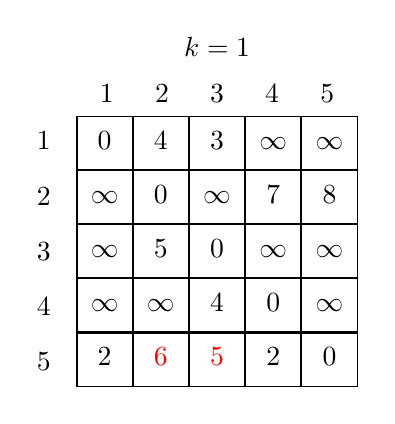
\begin{tikzpicture}
                \node at (-1.4,2) {1};
                \node at (-0.7,2) {2};
                \node at (0,2) {3};
                \node at (0.7,2) {4};
                \node at (1.4,2) {5};
                \node at (-2.2,1.4) {1};
                \node at (-2.2,0.7) {2};
                \node at (-2.2,0) {3};
                \node at (-2.2,-0.7) {4};
                \node at (-2.2,-1.4) {5};
                \node at (0,2.6) {$k = 1$};
                \matrix[matrix of nodes,nodes in empty cells,nodes={draw,text depth=.14cm, text height=.3cm, minimum width=.7cm}]
                {
                    0        & 4                  & 3                  & $\infty$ & $\infty$ \\
                    $\infty$ & 0                  & $\infty$           & 7        & 8        \\
                    $\infty$ & 5                  & 0                  & $\infty$ & $\infty$ \\
                    $\infty$ & $\infty$           & 4                  & 0        & $\infty$ \\
                    2        & \textcolor{red}{6} & \textcolor{red}{5} & 2        & 0        \\
                };
            \end{tikzpicture}
        \end{center}
    \end{minipage}
    \begin{minipage}[t]{0.5\textwidth}
        \begin{center}
            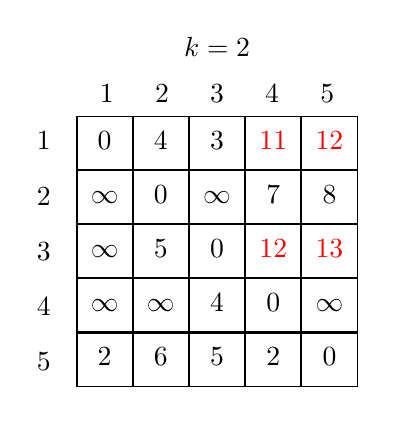
\begin{tikzpicture}
                \node at (-1.4,2) {1};
                \node at (-0.7,2) {2};
                \node at (0,2) {3};
                \node at (0.7,2) {4};
                \node at (1.4,2) {5};
                \node at (-2.2,1.4) {1};
                \node at (-2.2,0.7) {2};
                \node at (-2.2,0) {3};
                \node at (-2.2,-0.7) {4};
                \node at (-2.2,-1.4) {5};
                \node at (0,2.6) {$k = 2$};
                \matrix[matrix of nodes,nodes in empty cells,nodes={draw,text depth=.14cm, text height=.3cm, minimum width=.7cm}]
                {
                    0        & 4        & 3        & \textcolor{red}{11} & \textcolor{red}{12} \\
                    $\infty$ & 0        & $\infty$ & 7                   & 8                   \\
                    $\infty$ & 5        & 0        & \textcolor{red}{12} & \textcolor{red}{13} \\
                    $\infty$ & $\infty$ & 4        & 0                   & $\infty$            \\
                    2        & 6        & 5        & 2                   & 0                   \\
                };
            \end{tikzpicture}
        \end{center}
    \end{minipage}
    \begin{minipage}[t]{0.49\textwidth}
        \begin{center}
            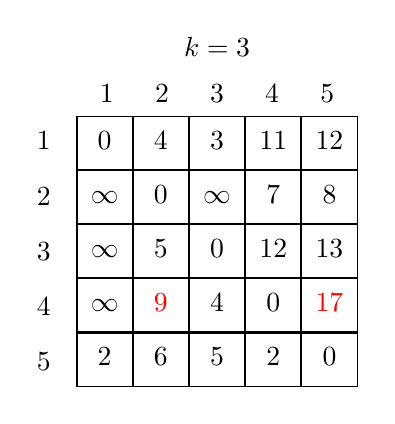
\begin{tikzpicture}
                \node at (-1.4,2) {1};
                \node at (-0.7,2) {2};
                \node at (0,2) {3};
                \node at (0.7,2) {4};
                \node at (1.4,2) {5};
                \node at (-2.2,1.4) {1};
                \node at (-2.2,0.7) {2};
                \node at (-2.2,0) {3};
                \node at (-2.2,-0.7) {4};
                \node at (-2.2,-1.4) {5};
                \node at (0,2.6) {$k = 3$};
                \matrix[matrix of nodes,nodes in empty cells,nodes={draw,text depth=.14cm, text height=.3cm, minimum width=.7cm}]
                {
                    0        & 4                   & 3        & 11       & 12                  \\
                    $\infty$ & 0                   & $\infty$ & 7        & 8                   \\
                    $\infty$ & 5                   & 0        & 12       & 13                  \\
                    $\infty$ & \textcolor{red}{9}  & 4        & 0        & \textcolor{red}{17} \\
                    2        & 6                   & 5        & 2        & 0                   \\
                };
            \end{tikzpicture}
        \end{center}
    \end{minipage}
    \begin{minipage}[t]{0.5\textwidth}
        \begin{center}
            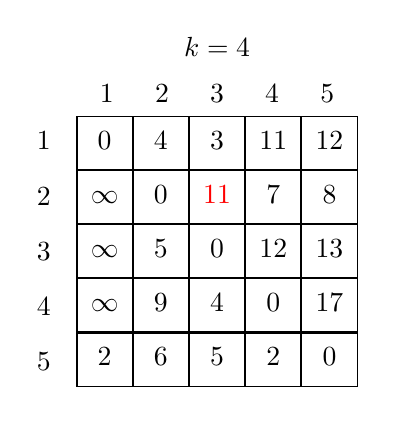
\begin{tikzpicture}
                \node at (-1.4,2) {1};
                \node at (-0.7,2) {2};
                \node at (0,2) {3};
                \node at (0.7,2) {4};
                \node at (1.4,2) {5};
                \node at (-2.2,1.4) {1};
                \node at (-2.2,0.7) {2};
                \node at (-2.2,0) {3};
                \node at (-2.2,-0.7) {4};
                \node at (-2.2,-1.4) {5};
                \node at (0,2.6) {$k = 4$};
                \matrix[matrix of nodes,nodes in empty cells,nodes={draw,text depth=.14cm, text height=.3cm, minimum width=.7cm}]
                {
                    0        & 4        & 3                   & 11       & 12       \\
                    $\infty$ & 0        & \textcolor{red}{11} & 7        & 8        \\
                    $\infty$ & 5        & 0                   & 12       & 13       \\
                    $\infty$ & 9        & 4                   & 0        & 17       \\
                    2        & 6        & 5                   & 2        & 0        \\
                };
            \end{tikzpicture}
        \end{center}
    \end{minipage}
    \begin{minipage}[t]{\textwidth}
        \begin{center}
            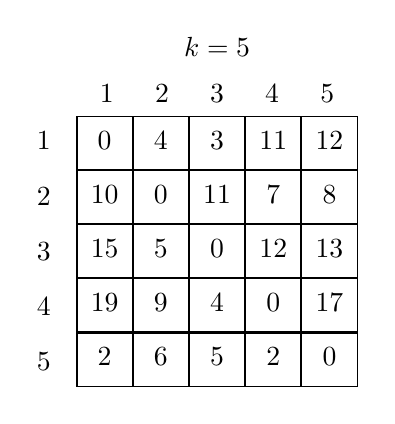
\begin{tikzpicture}
                \node at (-1.4,2) {1};
                \node at (-0.7,2) {2};
                \node at (0,2) {3};
                \node at (0.7,2) {4};
                \node at (1.4,2) {5};
                \node at (-2.2,1.4) {1};
                \node at (-2.2,0.7) {2};
                \node at (-2.2,0) {3};
                \node at (-2.2,-0.7) {4};
                \node at (-2.2,-1.4) {5};
                \node at (0,2.6) {$k = 5$};
                \matrix[matrix of nodes,nodes in empty cells,nodes={draw,text depth=.14cm, text height=.3cm, minimum width=.7cm}]
                {
                    0        & 4        & 3         & 11       & 12       \\
                    10       & 0        & 11        & 7        & 8        \\
                    15       & 5        & 0         & 12       & 13       \\
                    19       & 9        & 4         & 0        & 17       \\
                    2        & 6        & 5         & 2        & 0        \\
                };
            \end{tikzpicture}
        \end{center}
    \end{minipage}
\end{center}

Informațiile din matricea costurilor transformată prin algoritmul Roy-Floyd se ăpt folosi pentru a verifica dacă există drum cu costul minim între două noduri ale grafului, iar în caz afirmativ, se poate afișa lungimea lui și se poate descoperi drumul.

Algoritmul de transformare a matricei costurilor are ordinul de complexitate\textsuperscript{\cite{milosescu}} $O(n \cdot n \cdot n) = O(n^3)$, deoarece fiecare structură repetitivă \textbf{for} se execută de $n$ ori, iar structurile \textbf{for} sunt imbricate. Algoritmul de determinare a drumurilor cu costul minim din matricea costurilor transformată are ordinul de complexitate al algoritmului \textit{divide et impera}: $O(n \log n)$. Ordinul algoritmului este $O(n^3) + O(n \log n) = O(n^3 + n \log n) = O(n^3)$.

\subsection{Algoritmul Dijkstra}

Algoritmul lui Dijsktra\textsuperscript{\cite{milosescu}} construiește drumurile cu costul minim care pornesc de la un nod oarecare $x$, nodul sursă, până la fiecare nod din graful $G = (V, E)$, nodul destinație. Algoritmul întreține o mulțime cu nodurile care au fost deja selectate, $S$, și o coadă de priorități $Q$ cu nodurile care nu au fost selectate încă: $Q = V - S$, astfel:

\begin{itemize}
    \item Un nod $y$ este declarat selectat atunci când s-a determinat costul final al drumului cu costul minim de la nodul sursă $x$ la el. Selectarea unui nod nu este echivalentă cu găsirea drumului cu costul minim deoarece este posibil ca în urma calculării costului să rezulte că nu există drum de la nodul $x$ la acel nod.
    \item În coada $Q$ prioritatea cea mai mare o are nodul pentru care costul drumului are valoarea cea mai mică dintre toate costurile de drumuri care pornesc de la nodul $x$ la celelalte noduri selectate încă. La fiecare extragere a unui nod din coada de priorități $Q$, nodul este adăugat la mulțimea $S$, iar coada de priorități este reorganizată în funcție de acest nod. Pentru calcularea drumurilor de lungime minimă se întreține o mulțime $D$ în care se memorează costul drumurilor de la nodul $x$ la nodurile neselectate, costuri care se recalculează la fiecare extragere de nod.
\end{itemize}

Pentru implementarea algoritmului se folosesc trei vectori:
\begin{enumerate}
    \item Vectorul $s$ pentru mulțimea nodurilor selectate, definit astfel: 
    $$
        s_{i} =
        \begin{cases}
            0, & \text{dacă nodul } i \text{ nu a fost selectat} \\
            1, & \text{dacă nodul } i \text{ a fost selectat} \\
        \end{cases}.
    $$ Inițial, elementele vectorului $s$ au valoarea 0, cu excepția elementului $s_x$ care are valoarea 1. La terminarea execuției algoritmului, toate elementele din vectorul $s$ vor avea valoarea 1. Nodurile $i$ pentru care $s_i = 0$ se consideră că fac parte din coada de priorități $Q$.
    \item Vectorul $d$ conține costul drumurilor, astfel: $d_i$ este costul drumului minim găsit la un moment dat de la nodul $x$ la nodul $i$, cu $i \in \overline{1, n}$. Inițial $d_i = a_{x,i}$. La terminarea algoritmului, $d_{i}$ este costul minim al drumului de la nodul $x$ la nodul $i$.
    \item Vectorul $t$ memorează drumurile găsite între nodul $x$ și celelalte noduri $i$ ale grafului. Memorarea drumului se face prin legătura cu predecesorul are este definită astfel: $p_i$ memorează nodul $j$ care este predecesorul nodului $i$ pe drumul de la $x$, cu excepția nodului sursă pentru care $p_x = 0$. Inițial, pentru toate nodurile $i$ care nu au costul infinit (pentru care există un arc de la nodul $x$ la nodul $i$), $p_i = x$; altfel $p_i = 0$.
\end{enumerate}

Nodul $i$ care se extrage din coada de priorități $Q$ trebuie să îndeplinească următoarele condiții:
\begin{itemize}
    \item $s_i = 0$
    \item $d_i = \min{(d_j | 1 \leq j \leq n; s_j = 0)}$.
\end{itemize}

Pentru graful din figura \ref{fig:graf4}, considerând $x = 1$, algoritmul se execută astfel:

\textbf{Inițial:}
\begin{center}
    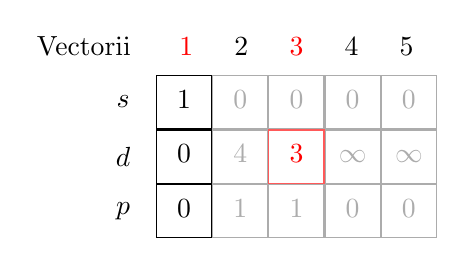
\begin{tikzpicture}
        \node at (-1.4,1.4) {\textcolor{red}{1}};
        \node at (-0.7,1.4) {2};
        \node at (0,1.4) {\textcolor{red}{3}};
        \node at (0.7,1.4) {4};
        \node at (1.4,1.4) {5};
        \node at (-2.7,1.4) {Vectorii};
        \node at (-2.2,0.7) {$s$};
        \node at (-2.2,0) {$d$};
        \node at (-2.2,-0.7) {$p$};
        \matrix[matrix of nodes,nodes in empty cells,nodes={draw,text depth=.14cm, text height=.3cm, minimum width=.7cm}]
        {
            1 & |[gray!65]|0 & |[gray!65]|0                 & |[gray!65]|0        & |[gray!65]|0        \\
            0 & |[gray!65]|4 & |[red!65]|\textcolor{red}{3} & |[gray!65]|$\infty$ & |[gray!65]|$\infty$ \\
            0 & |[gray!65]|1 & |[gray!65]|1                 & |[gray!65]|0        & |[gray!65]|0        \\
        };
    \end{tikzpicture}
\end{center}

Drumul cu costul cel mai mic este cu nodul $3$: $d_3 = 3$. Nodul $3$ se va extrage din coada $Q$. Se analizează nodurile care rămân în coada de priorități.

Nodul $2$: $d_3 + a_{3,2} = 3 + 5 = 8 > 4$. Nu se modifică nimic.

Nodul $4$: $d_3 + a_{3,4} = 3 + \infty = \infty > 4$. Nu se modifică nimic.

Nodul $5$: $d_3 + a_{3,5} = 3 + \infty = \infty > 4$. Nu se modifică nimic.

\begin{center}
    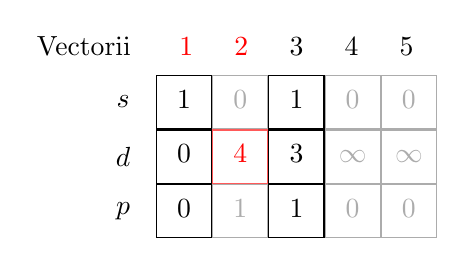
\begin{tikzpicture}
        \node at (-1.4,1.4) {\textcolor{red}{1}};
        \node at (-0.7,1.4) {\textcolor{red}{2}};
        \node at (0,1.4) {3};
        \node at (0.7,1.4) {4};
        \node at (1.4,1.4) {5};
        \node at (-2.7,1.4) {Vectorii};
        \node at (-2.2,0.7) {$s$};
        \node at (-2.2,0) {$d$};
        \node at (-2.2,-0.7) {$p$};
        \matrix[matrix of nodes,nodes in empty cells,nodes={draw,text depth=.14cm, text height=.3cm, minimum width=.7cm}]
        {
            1 & |[gray!65]|0                  & 1 & |[gray!65]|0        & |[gray!65]|0       \\
            0 & |[red!65]|\textcolor{red}{4} & 3 & |[gray!65]|$\infty$ & |[gray!65]|$\infty$ \\
            0 & |[gray!65]|1                  & 1 & |[gray!65]|0        & |[gray!65]|0       \\
        };
    \end{tikzpicture}
\end{center}

Drumul cu costul cel mai mic este cu nodul $2$: $d_2 = 4$. Nodul $2$ se va extrage din coada $Q$. Se analizează nodurile care rămân în coada de priorități.

Nodul $4$: $d_2 + a_{2,4} = 4 + 7 = 11 < \infty$. Se modifică: $d_4 = 11$ și $p_4 = 2$.

Nodul $5$: $d_2 + a_{2,5} = 4 + 8 = 12 < \infty$. Se modifică: $d_5 = 12$ și $p_5 = 2$.

\begin{center}
    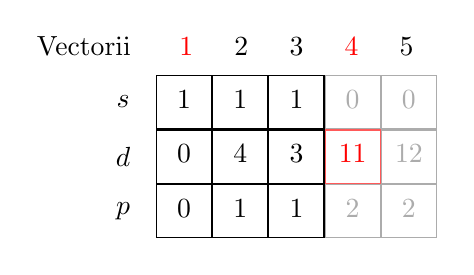
\begin{tikzpicture}
        \node at (-1.4,1.4) {\textcolor{red}{1}};
        \node at (-0.7,1.4) {2};
        \node at (0,1.4) {3};
        \node at (0.7,1.4) {\textcolor{red}{4}};
        \node at (1.4,1.4) {5};
        \node at (-2.7,1.4) {Vectorii};
        \node at (-2.2,0.7) {$s$};
        \node at (-2.2,0) {$d$};
        \node at (-2.2,-0.7) {$p$};
        \matrix[matrix of nodes,nodes in empty cells,nodes={draw,text depth=.14cm, text height=.3cm, minimum width=.7cm}]
        {
            1 & 1 & 1 & |[gray!65]|0                   & |[gray!65]|0 \\
            0 & 4 & 3 & |[red!65]|\textcolor{red}{11} & |[gray!65]|12 \\
            0 & 1 & 1 & |[gray!65]|2                   & |[gray!65]|2 \\
        };
    \end{tikzpicture}
\end{center}

Drumul cu costul cel mai mic este cu nodul $4$: $d_4 = 11$. Nodul $4$ se va extrage din coada $Q$. Se analizează nodurile care rămân în coada de priorități.

Nodul $5$: $d_4 + a_{4,5} = 11 + \infty = \infty > 12$. Nu se modifică nimic.

\begin{center}
    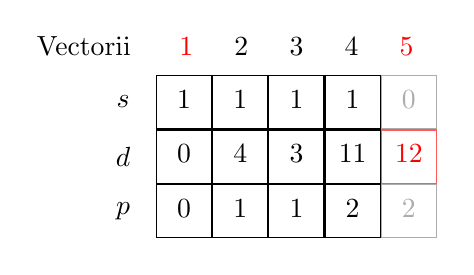
\begin{tikzpicture}
        \node at (-1.4,1.4) {\textcolor{red}{1}};
        \node at (-0.7,1.4) {2};
        \node at (0,1.4) {3};
        \node at (0.7,1.4) {4};
        \node at (1.4,1.4) {\textcolor{red}{5}};
        \node at (-2.7,1.4) {Vectorii};
        \node at (-2.2,0.7) {$s$};
        \node at (-2.2,0) {$d$};
        \node at (-2.2,-0.7) {$p$};
        \matrix[matrix of nodes,nodes in empty cells,nodes={draw,text depth=.14cm, text height=.3cm, minimum width=.7cm}]
        {
            1 & 1 & 1 & 1  & |[gray!65]|0                  \\
            0 & 4 & 3 & 11 & |[red!65]|\textcolor{red}{12} \\
            0 & 1 & 1 & 2  & |[gray!65]|2                  \\
        };
    \end{tikzpicture}
\end{center}

Drumul cu costul cel mai mic este cu nodul $5$: $d_5 = 15$. Nodul $5$ se va extrage din coada $Q$. Coada este vidă și se termină execuția algoritmului.

\textbf{Final:}
\begin{center}
    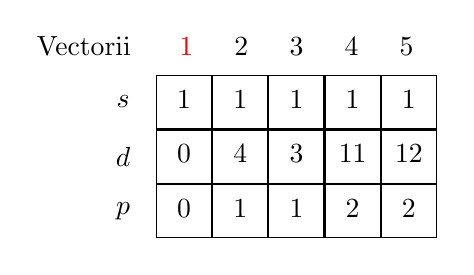
\begin{tikzpicture}
        \node at (-1.4,1.4) {\textcolor{red}{1}};
        \node at (-0.7,1.4) {2};
        \node at (0,1.4) {3};
        \node at (0.7,1.4) {4};
        \node at (1.4,1.4) {5};
        \node at (-2.7,1.4) {Vectorii};
        \node at (-2.2,0.7) {$s$};
        \node at (-2.2,0) {$d$};
        \node at (-2.2,-0.7) {$p$};
        \matrix[matrix of nodes,nodes in empty cells,nodes={draw,text depth=.14cm, text height=.3cm, minimum width=.7cm}]
        {
            1 & 1 & 1 & 1  & 1  \\
            0 & 4 & 3 & 11 & 12 \\
            0 & 1 & 1 & 2  & 2  \\
        };
    \end{tikzpicture}
\end{center}

Din datele care se găsesc în vectorii $d$ și p la terrminarea algoritmului se obțin următoarele informații:

\begin{itemize}
    \item $d_i$ reprezintă costul minim al drumului de la nodul $x$ la nodul $i$. De exemplu, pentru nodul $4$ costul minim este $11$.
    \item Din vectorul predecesorilor se reconstituie drumul cu costul minim de la nodul $x$ la nodul $i$. De exemplu, pentru nodul 4: $p_4 = 2$, iar $p_2 = 1$. Drumul este $1 \rightarrow 2 \rightarrow 4$.
\end{itemize}

\begin{thebibliography}{9}
    \bibitem{gabow}
    Harold N. Gabow.
    \href{https://www.cs.colorado.edu/~hal/Papers/DFS/alldfs.pdf}{\textit{Graph Theory Definitions}}.
    The Department of Computer Science at the University of Colorado Boulder, 2008.

    \bibitem{milosescu}
    Mariana Miloșescu.
    \textit{Informatică intensiv: C++: manual pentru clasa a XI-a, ed. a 3-a}.
    Editura Didactică și Pedagogică, 2012.

    \bibitem{andonie}
    Răzvan Andonie, Ilie Gârbacea.
    \textit{Algoritmi fundamentali. O perspectivă C++}.
    Editura Libris, Cluj-Napoca, 2012.
\end{thebibliography}

\end{document}